\subsection{3D wing inverse design case}
\label{ch7:sect:wingCase}
In this section, we employ the generative inverse model to explore high aerodynamic performance wing candidates for the three-dimensional wing shape design. It is worth mentioning that our generative model is not used to solve a design optimization problem in this case; instead, it is used to generate desired design candidates under given constraints. 
Referring to the American Institute of Aeronautics and Astronautics (AIAA) Aerodynamic Design Optimization Discussion Group (ADODG)\footnote{AIAA ADODG webpage: \url{https://sites.google.com/view/mcgill-computational-aerogroup/adodg} (last accessed on 26 July 2025).} case 4.1 and previous benchmark investigations~\cite{aa.Lyu2015,aa.Li2021c}, we set the multi-dimensional constraints to the generative model to achieve lift-to-drag ratio $L/D = 21.8$, which is the highest performance achieved using adjoint CFD solver (specifically by a design with $C_{L} = 0.5$ and $C_{D} = 0.0229$). 

We further validate the wing samples using ADflow~\cite{aa.Mader2020,aa.Kenway2019}\footnote{ADflow repository: \url{https://github.com/mdolab/adflow.git} (last access on 26 July 2025)} CFD solver and visualize the pressure coefficient $C_{P}$ distributions of two samples as shown in Figure~\ref{ch7:fig:wingAerodynamic}. From the $C_P$ distributions, it is evident that, relative to conventional methods, \textit{Dflow-SUR} produces more aerodynamically-coherent shapes, yielding a more uniform $C_P$ variation from the leading edge to the trailing edge.

\begin{figure}[ht!]
    \centering
    \subfloat[Wing sample generated using LHS]{%
        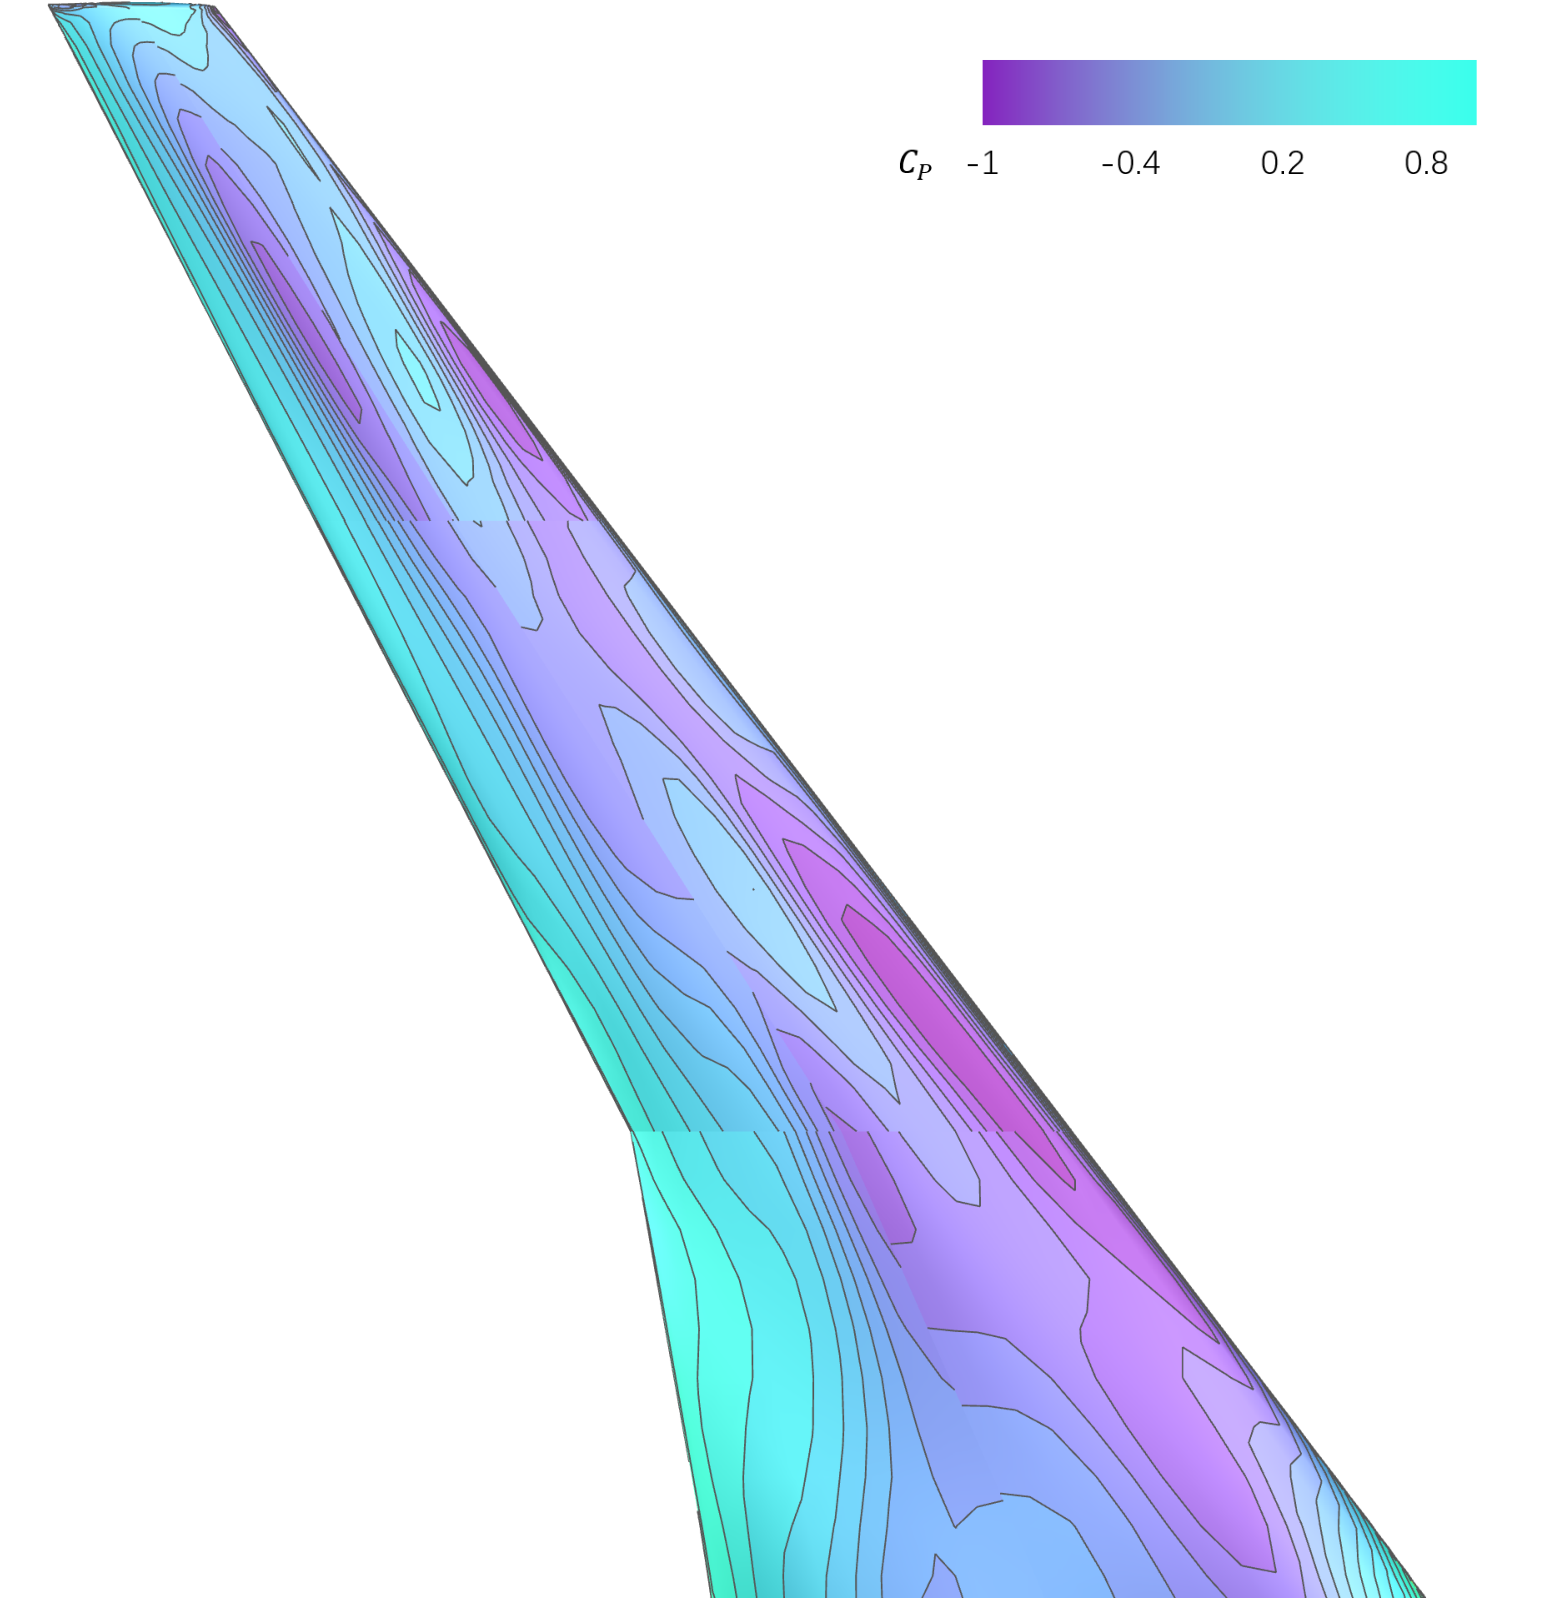
\includegraphics[width=0.5\textwidth]{chapter7/fig/LHS.pdf}%
    }\hfill
    \subfloat[Wing sample generated using Dflow-SUR]{%
        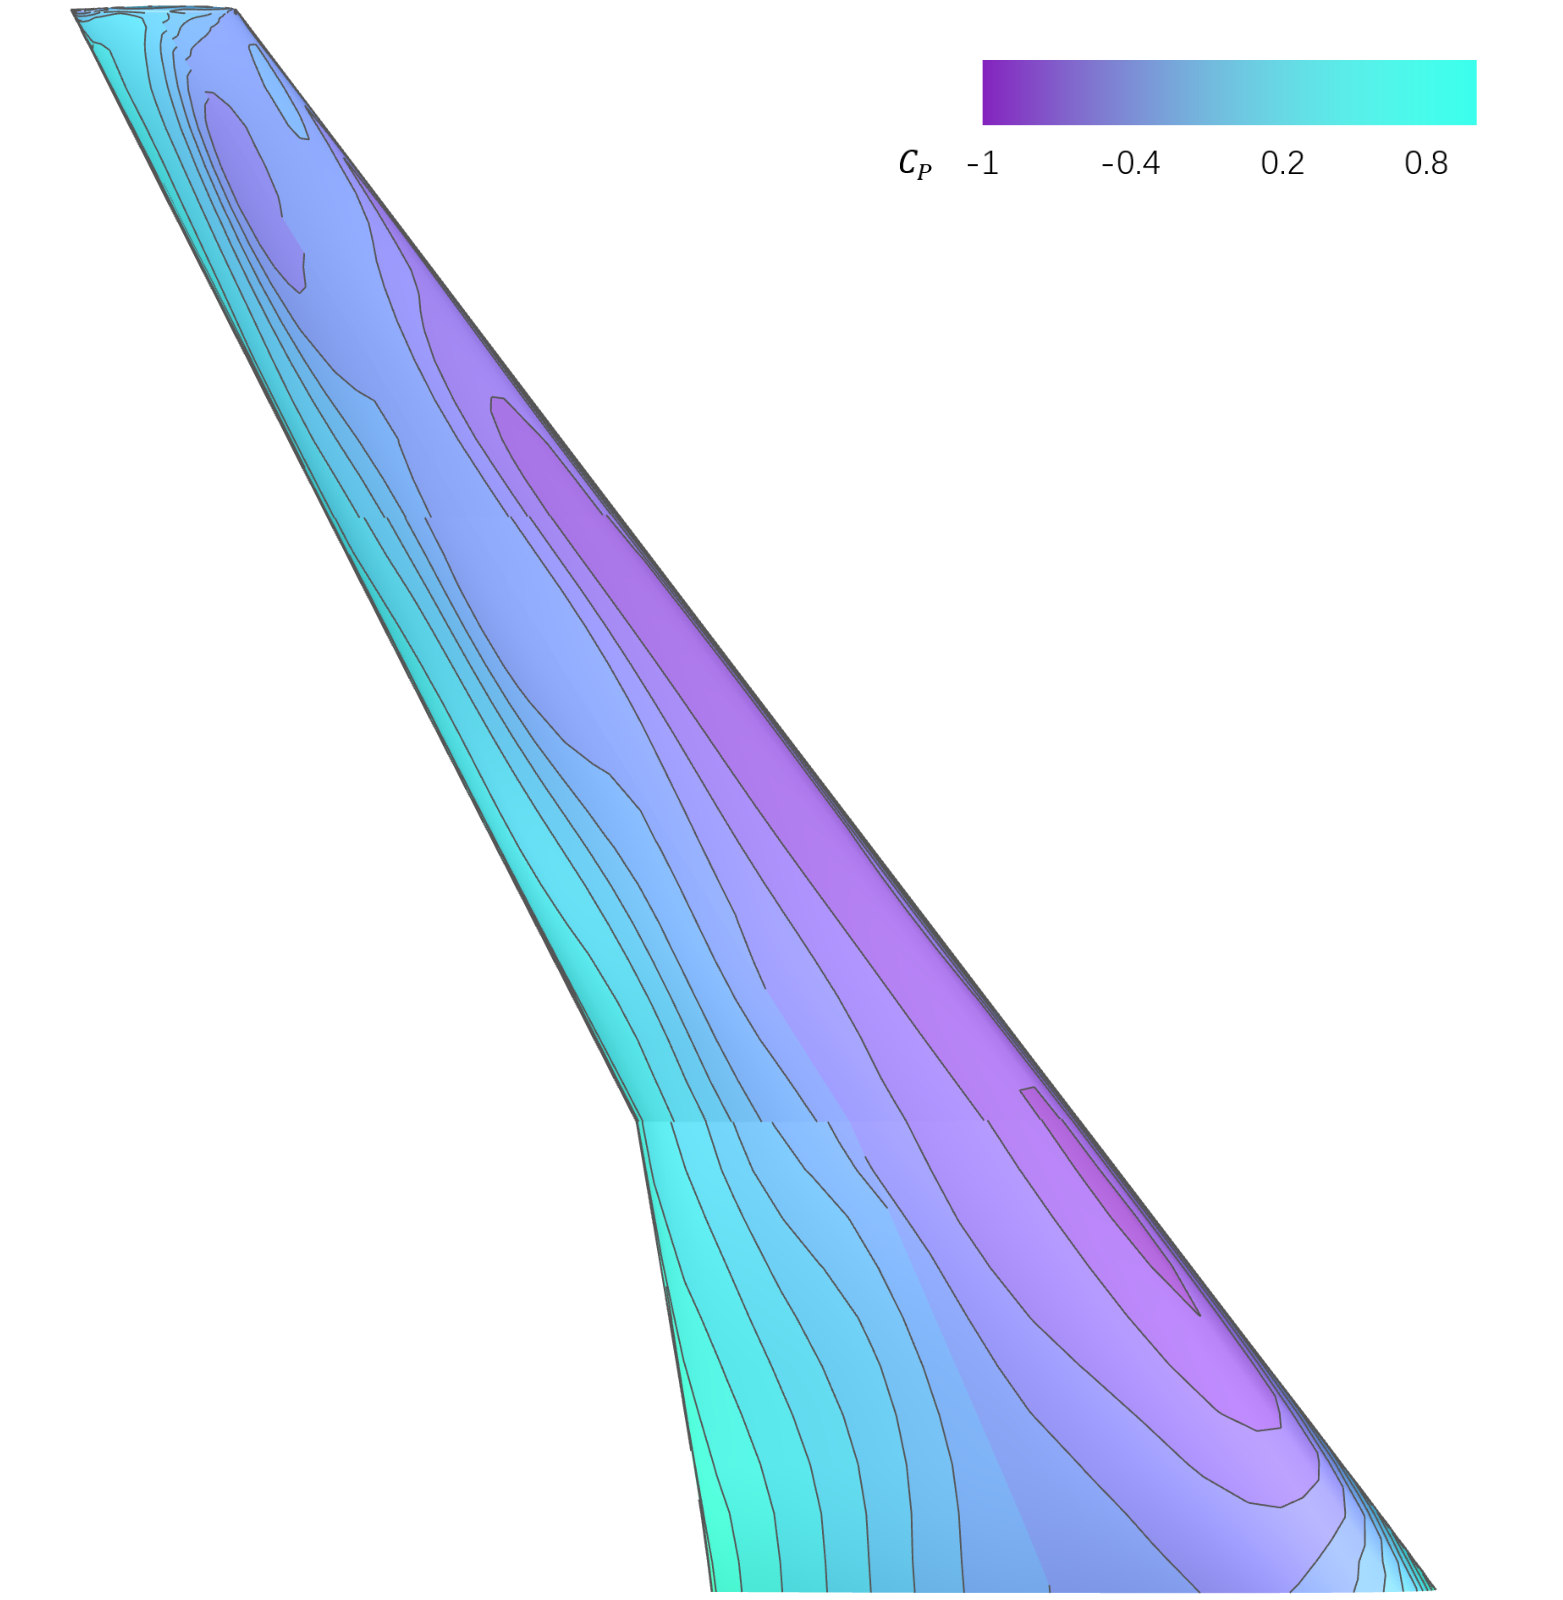
\includegraphics[width=0.5\textwidth]{chapter7/fig/Dflow_SUR.pdf}%
    }
    \caption{Wing sample $C_{P}$ distribution validated using ADflow.}
    \label{ch7:fig:wingAerodynamic}
\end{figure}

Figure~\ref{ch7:fig:wingPerformance} shows the probability density (Figure~\ref{ch7:subfig:wing_PDF}) and violin plot (Figure~\ref{ch7:subfig:wing_violin}) of wing samples' $L/D$ distributions using LHS, energy-based, and \textit{Dflow-SUR} approaches. The data shown herein are truncated at its observed minimum and maximum values. From the results, \textit{Dflow-SUR} outperforms both LHS and the energy-based approach as a sampling method: it achieves a higher mean $L/D$ ($21.1845$ as compared to $18.3998$ obtained using LHS and $19.8416$ from the energy-based approach) and a lower standard deviation ($0.7020$ as compared to $1.4641$ and $1.0201$ obtained using LHS and the energy-based approach, respectively). This indicates that \textit{Dflow-SUR} not only shifts the distribution toward higher aerodynamic performance but also concentrates design candidates more tightly around higher $L/D$ values, yielding a more efficient generation of high-performance geometries.
\begin{figure}[ht!]
    \centering
    \subfloat[Probability density plot]{%
        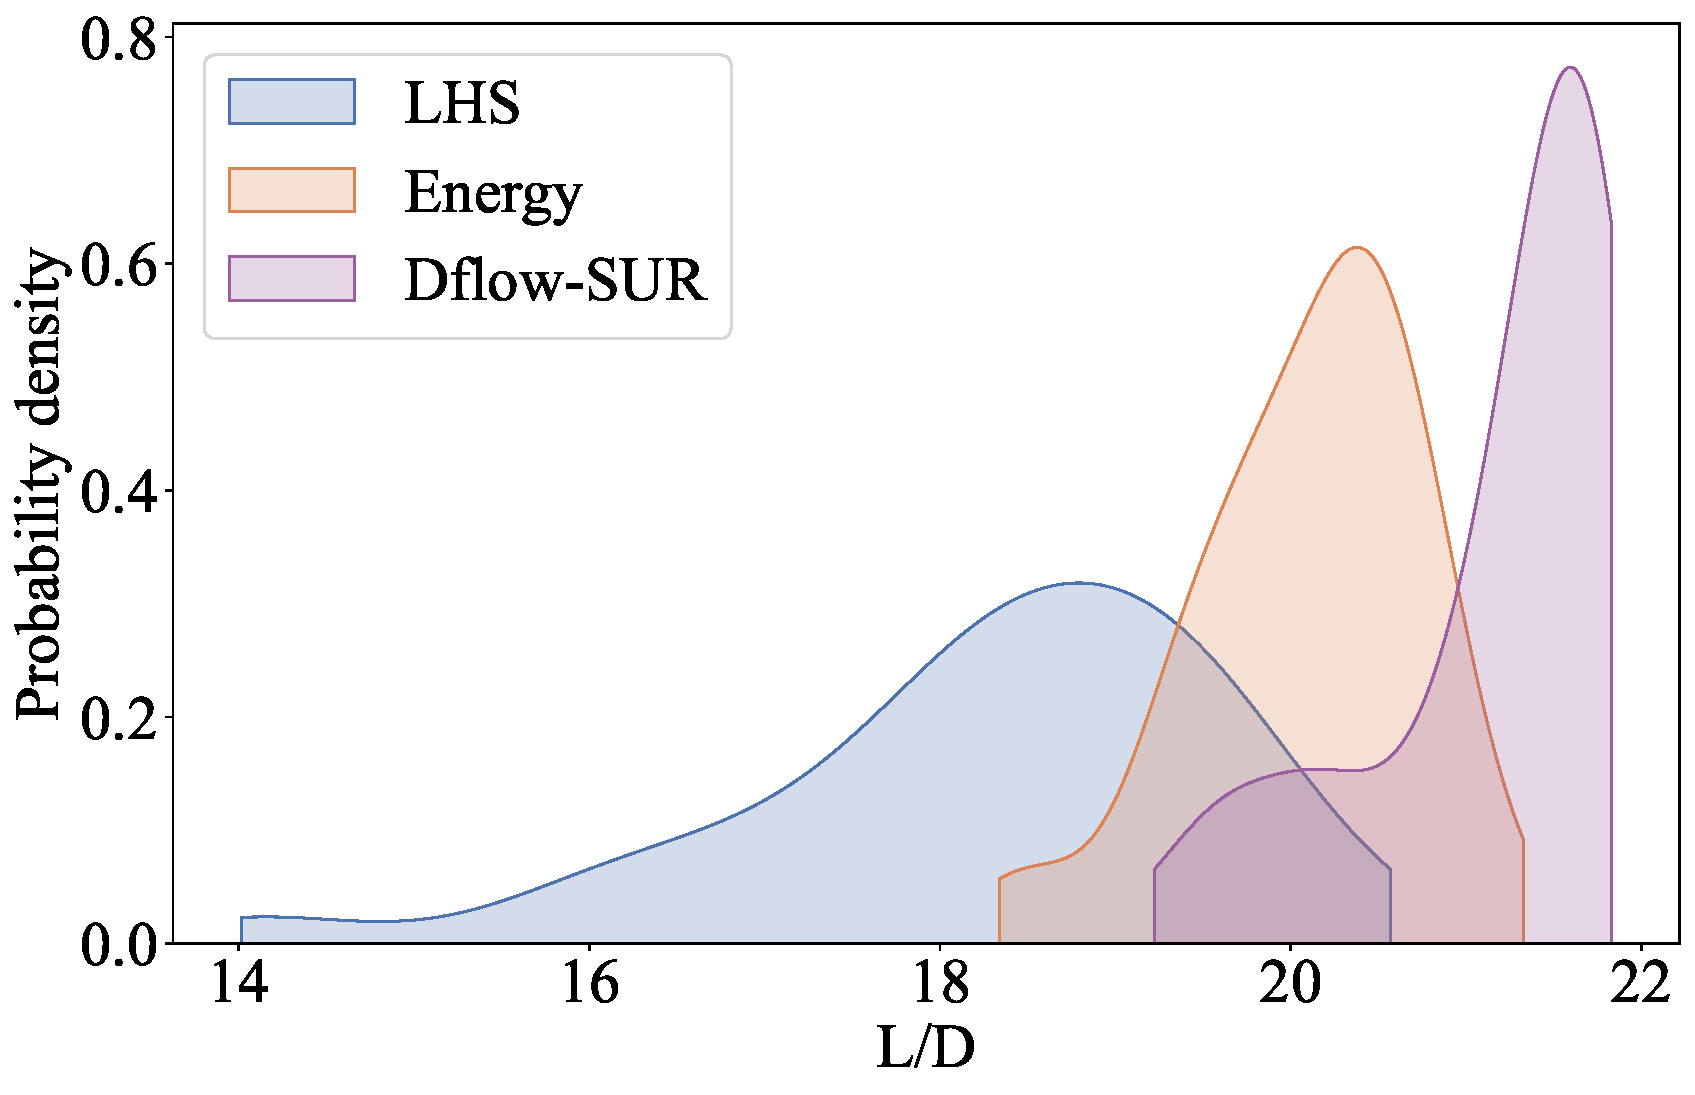
\includegraphics[width=0.65\textwidth]{chapter7/fig/probability_density_plot.pdf}%
        \label{ch7:subfig:wing_PDF}
    }\\[1em]
    \subfloat[Violin plot]{%
        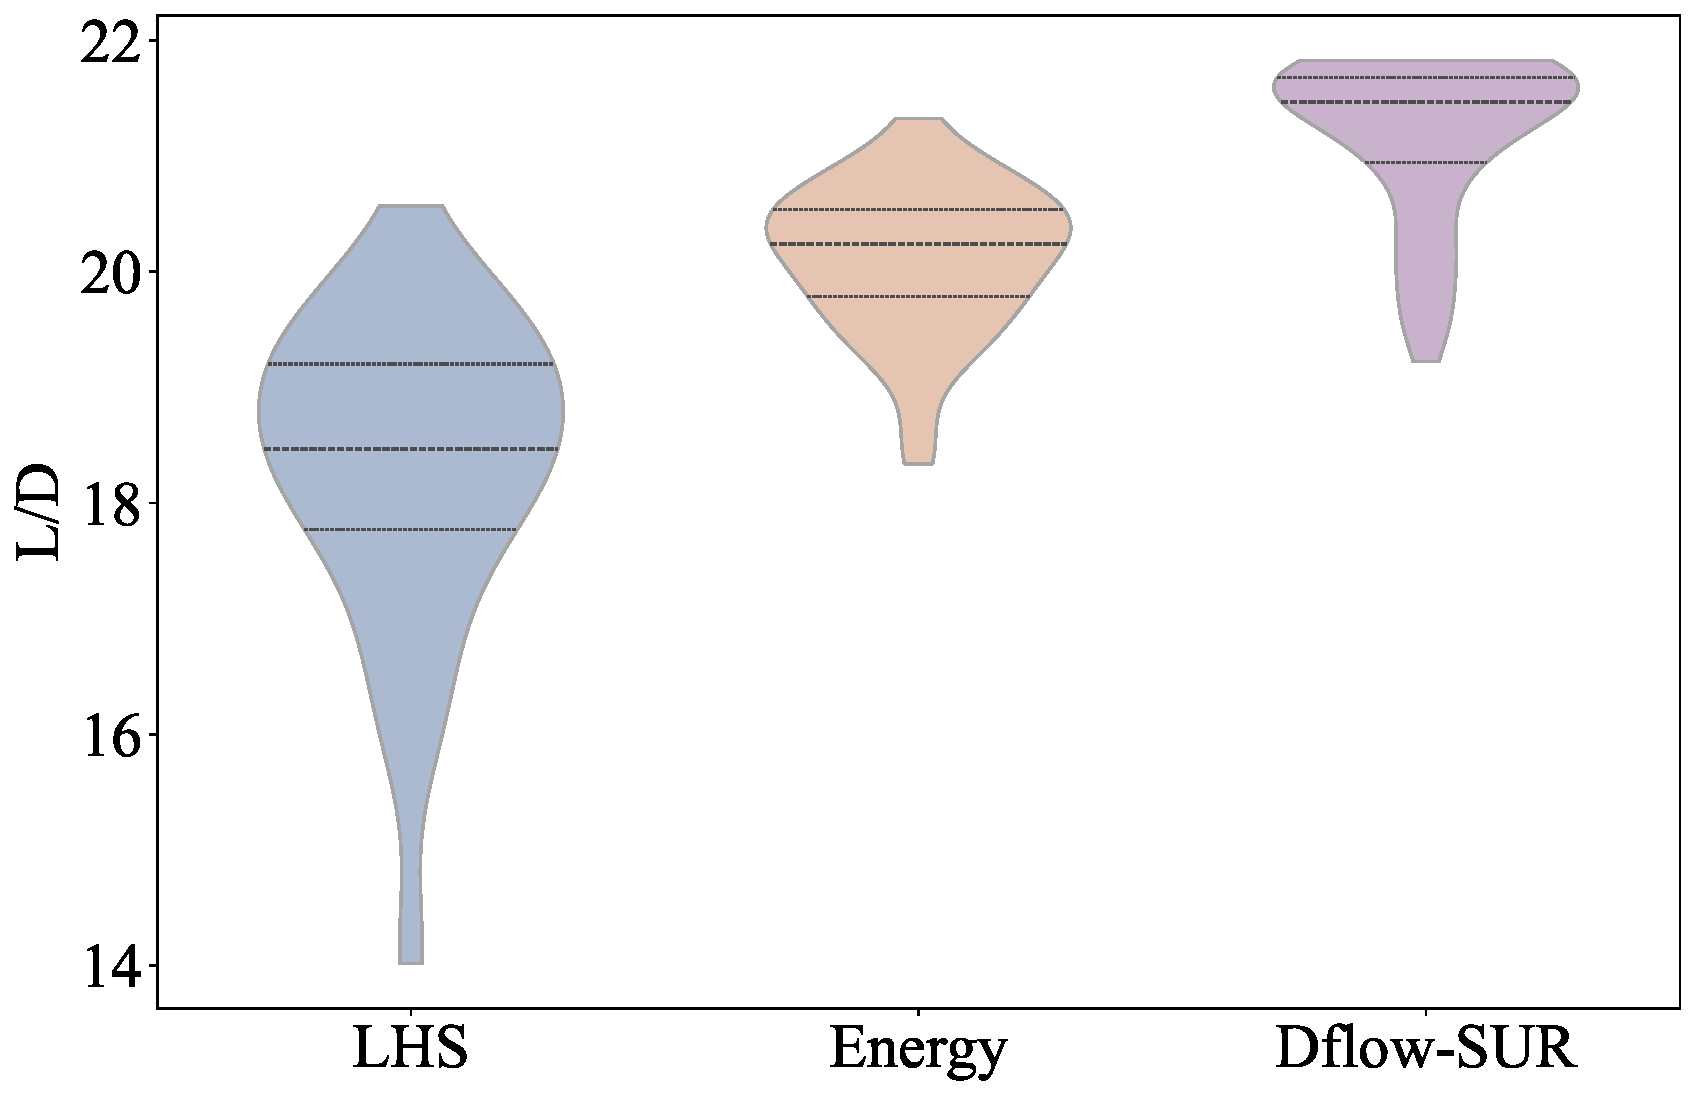
\includegraphics[width=0.65\textwidth]{chapter7/fig/violin_plot_equal_area.pdf}%
        \label{ch7:subfig:wing_violin}
    }\\[1em]

    \caption{Probability density and violin plot of wing samples $L/D$ distribution using three sampling approaches. (Three horizontal lines in each violin plot indicate the 25th percentile, median, and 75th percentile.)}
    \label{ch7:fig:wingPerformance}
\end{figure}

The wing samples and surrogate model are validated in a previous work by Li and Zhang~\cite{aa.Li2021b}, which were used to perform surrogate-based wing shape optimization of the Common Research Model (CRM) wing\footnote{NASA Common Research Model (CRM) webpage: \url{https://commonresearchmodel.larc.nasa.gov/} (last accessed on 26 July 2025).}. The wing samples are generated via Latin Hypercube Sampling (LHS) around the CRM wing baseline shape using a compact modal parameterization method, which is also based on another work by Li and Zhang~\cite{aa.Li2021c}. The surrogate model on aerodynamic estimation is built with inputs of wing geometry $\mathbf{x}$, wing twists $\alpha_{twist}$, Mach number $M$, flight altitude $h$, angle of attack $\alpha$ and outputs $C_{L}$, $C_{D}$ and $C_{M}$. 

It is worth noting that this study focuses on investigating how to better integrate physical guidance into flow models. The performance of the resulting generative model depends on the accuracy of the surrogate model, which may lead to discrepancies with respect to CFD solutions. However, this issue pertains to the broader discussion between surrogate models and CFD, falling outside the scope of the present study.


